\documentclass[a4paper; 11pt]{article}
\usepackage[utf8]{inputenc}
\usepackage[english]{babel}
\usepackage{graphicx}
\usepackage{multicol}
\makeatletter
\setlength{\@fptop}{0pt}
\makeatother
\setlength{\columnsep}{1cm}
\bibliographystyle{unsrt}
\begin{document}

\title{Usability of Mobile Map Applications}

\author{Rachel Rivera\\
Professor: Dr. Dionisio\\
CMSI 370: Interaction Design\\
  Loyola Marymount University}

\date{September 25, 2014}

% Create title page with no page number

\renewcommand{\thefootnote}{\fnsymbol{footnote}}



%\singlespacing

\maketitle

\vspace{-.2in}
\begin{center}
\begin{abstract}
\noindent This investigation is motivated by the increasing significance of the usability of systems in today's competitive technology market. Usability testing and usability evaluations have become important tools in the assessment of user interfaces. This paper presents empirical mobile usability studies of two distinct map applications: Google Maps and Apple Maps. Participants of this investigation were asked to carry out three tasks with each mobile application. The results of this examination include (a) the contextual factors studied; (b) quantitative data collected from each task; (c) a brief qualitative review from each participant; and (d) the core usability metrics measured. This paper not only presents the usability metrics collected by the study but also presents a heuristic evaluation of each map application.
\end{abstract}
\end{center}

\medskip
\medskip


\medskip
\noindent \textit{Group Members}: Katarina Klask, J.B. Morris, Alex Schneider, Khalid Seirafi, and Ronald Uy.

\thispagestyle{empty}

\clearpage

%\onehalfspacing
\setcounter{footnote}{0}
\renewcommand{\thefootnote}{\arabic{footnote}}
\setcounter{page}{1}

\section{Introduction}
When the Apple Maps mobile application was first released as part of iOS 6 in September 2012, it received a significant amount of negative feedback. Walt Mossberg of the \textit{Wall Street Journal} was one of many who thought that Apple Maps was the biggest drawback of the iPhone 5.\cite{Mossberg} At this time, the Google Maps mobile apps, on both iOS and Android, were used by roughly 81 million people.\cite{ComScore} However, Apple Maps grew, matured, and began gaining traction. By September 2013, Apple Maps gained 35 million regular users. The number of users of Google Maps dropped to around 58.7 million at this time.\cite{ComScore} Although the Apple Maps mobile app is newer than the Google Maps mobile app,\footnote{The initial release of Google Maps for Mobile was in September of 2008.} the two map applications are comparable with respect to features they provide as well as popularity nowadays.
\medskip
\par
Since both Google Maps apps and Apple Maps apps are widely known and used, it is important that the usability metrics of the two systems are examined. Thus, this study aims to empirically investigate the usability of each application. The current consensus within the field of interaction design is that usability depends on five distinct metrics: \textit{learnability}, \textit{efficiency}, \textit{errors}, \textit{memorability}, and \textit{satisfaction}.\cite{Nielsen} The three metrics that this particular study focuses on are efficiency, errors, and satisfaction.
\section{The Experiment} \label{sec:Experiment}
Each person who participated in this study had to carry out three concrete tasks with each of the map applications.
\begin{enumerate}
  \item Save a pin anywhere on the map and get driving directions to that pin.
  \item Find the location of the nearest Vons.
  \item Find the fastest route from the current location to LACMA.
\end{enumerate}
In order to keep the study as controlled as possible, all testing was done on iOS devices (no map applications of android devices were tested). As test subjects executed the tasks, information was collected pertaining to their efficiency, errors, and satisfaction.

\subsection{Contextual Factors}
Prior to having each test subject perform the tasks, a little contextual data about the users was first collected. Users were asked about their previous experience with Apple Maps, their previous experience with Google Maps, and their overall technological proficiency.
\clearpage

One problem that arose when conducting this study was that almost every test subject had significantly more Google Maps experience than Apple Maps experience. This is not necessarily surprising since Apple Maps is a newer application. However, this study was aiming to test efficiency, and not learnability. Thus if a test subject did not have any experience with an application, the test subject would not be asked to execute tasks on that application.

\begin{figure}[ht]
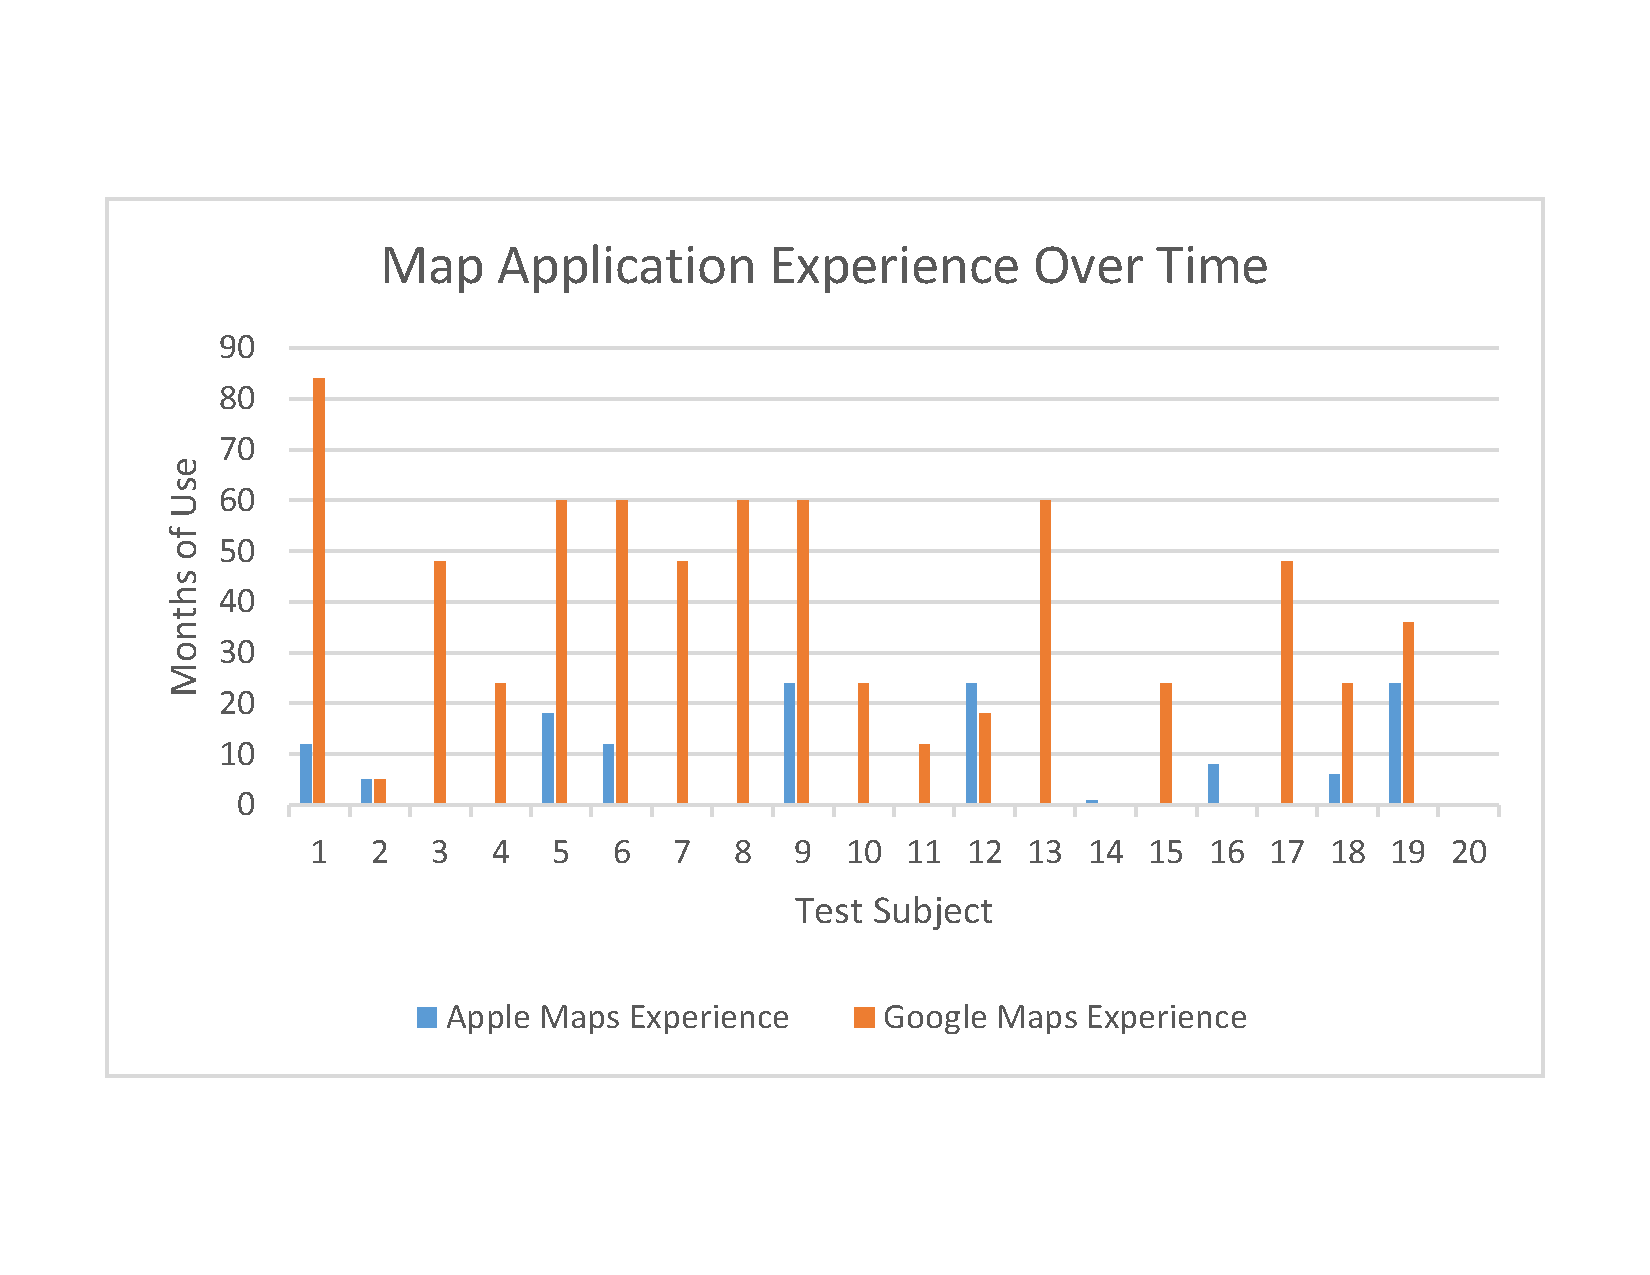
\includegraphics[keepaspectratio, width=1\textwidth ]{user_context.pdf}
\end{figure}

\subsection{Results}
\textit{The design of system icons is simple, modern, friendly, and sometimes quirky. Each icon is reduced to its minimal form, with every idea edited to its essence. The designs ensure readability and clarity even at small sizes}
\begin{figure}[ht]
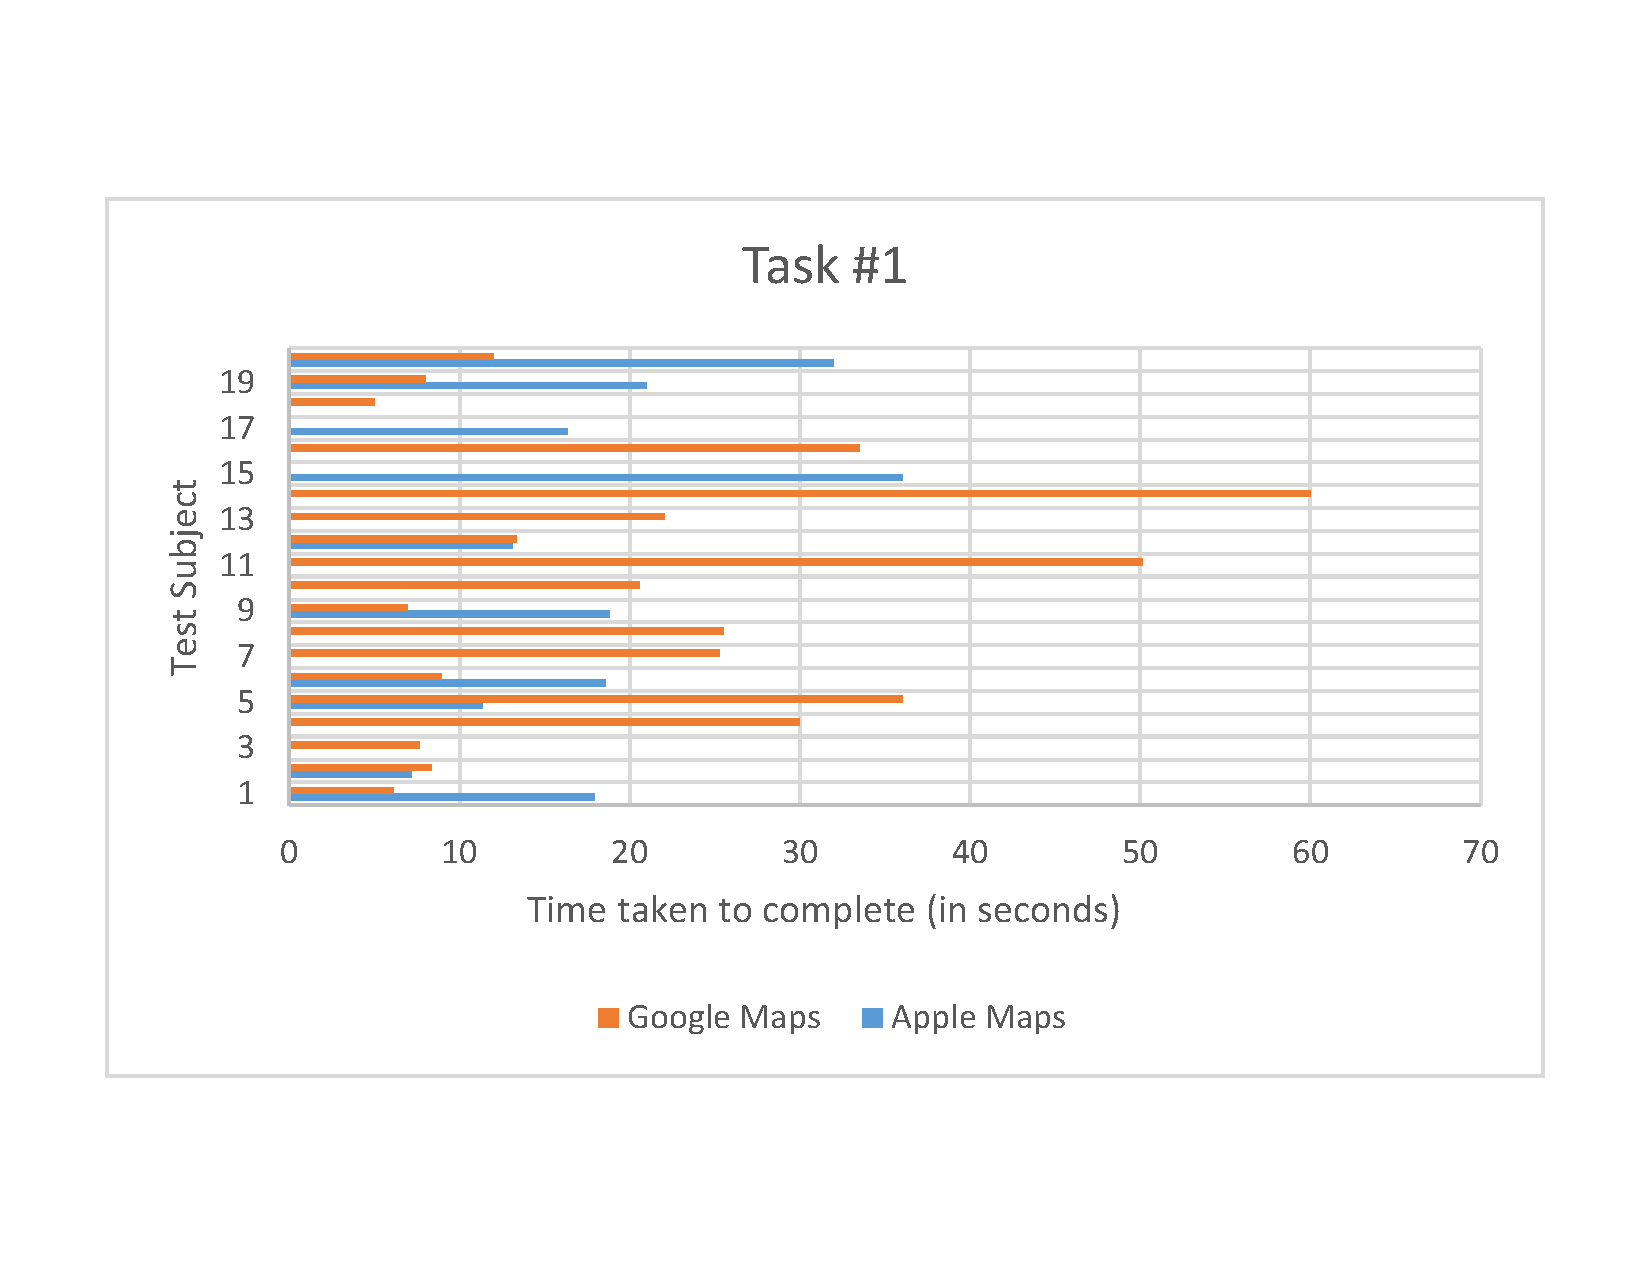
\includegraphics[keepaspectratio, width=1\textwidth ]{task1.pdf}
\end{figure}
\begin{figure}[ht]
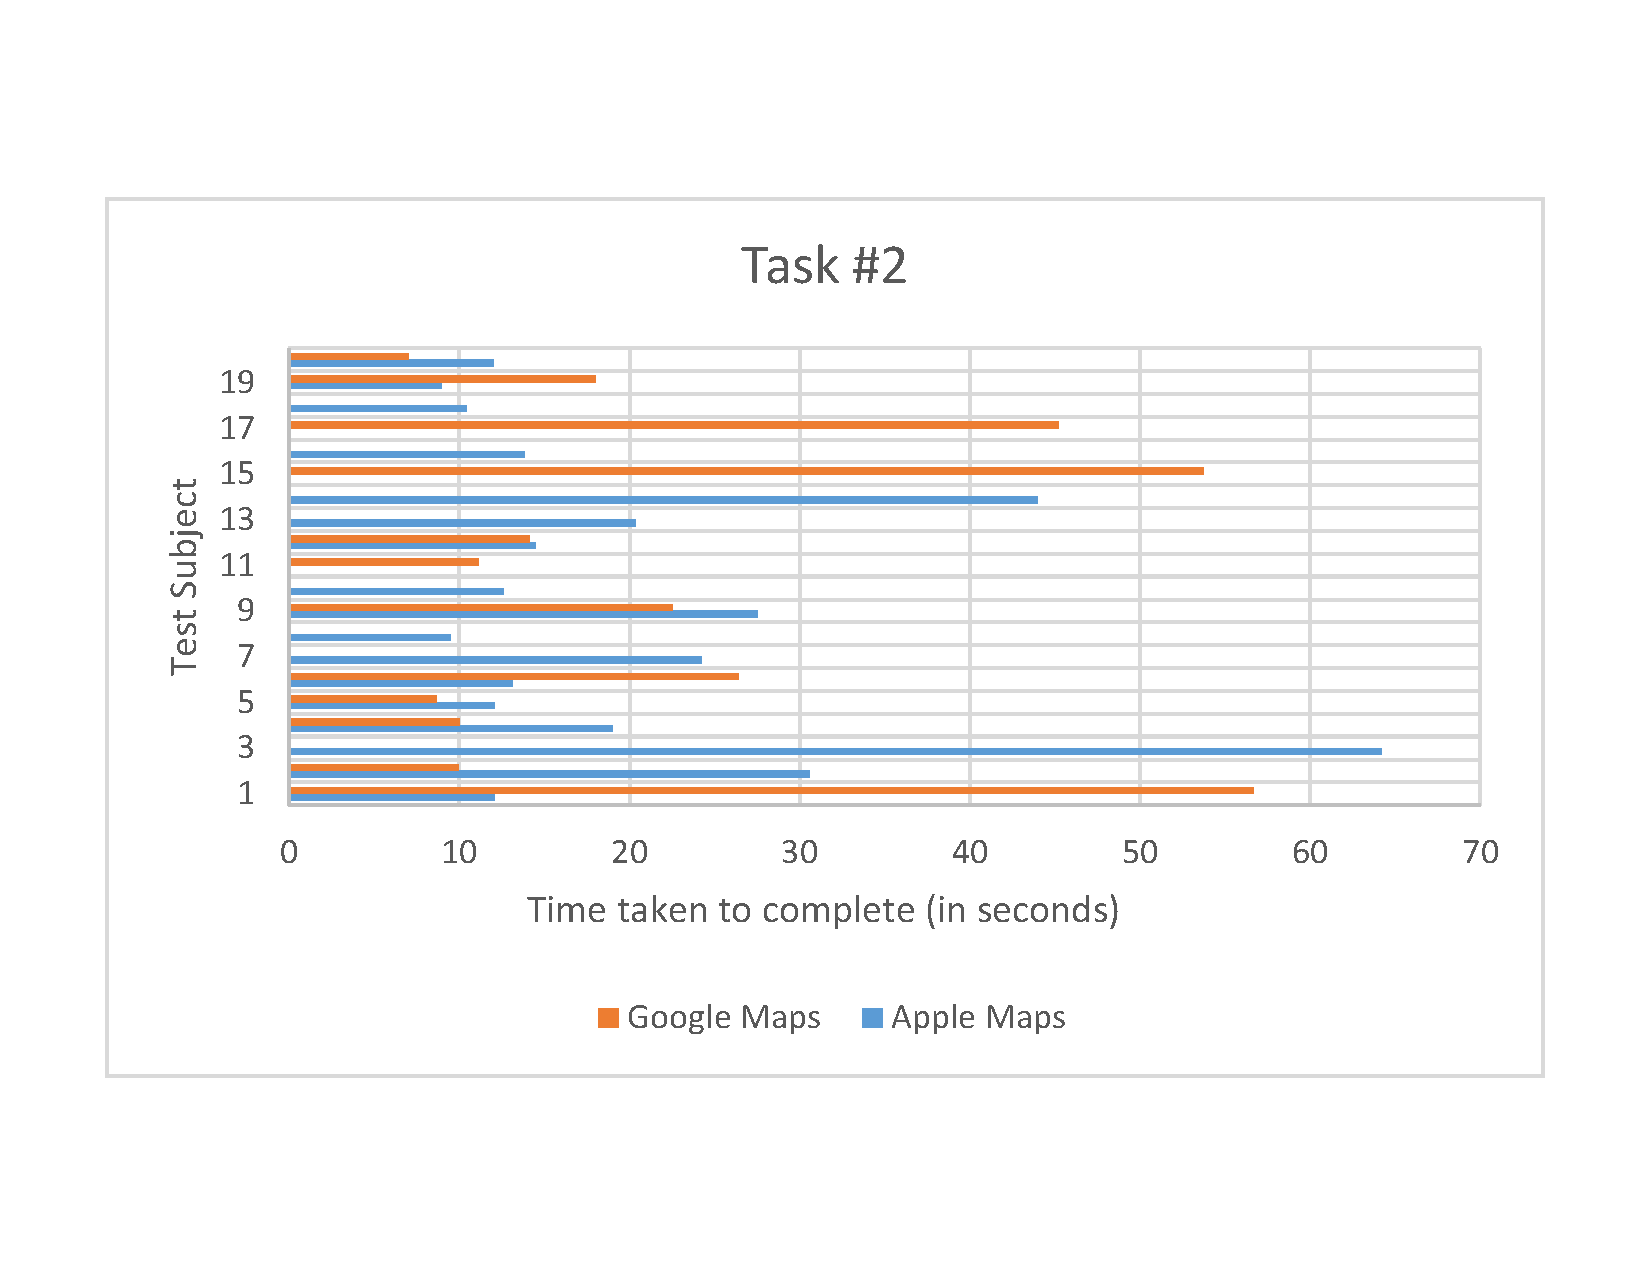
\includegraphics[keepaspectratio, width=1\textwidth ]{task2.pdf}
\end{figure}
\begin{figure}[ht]
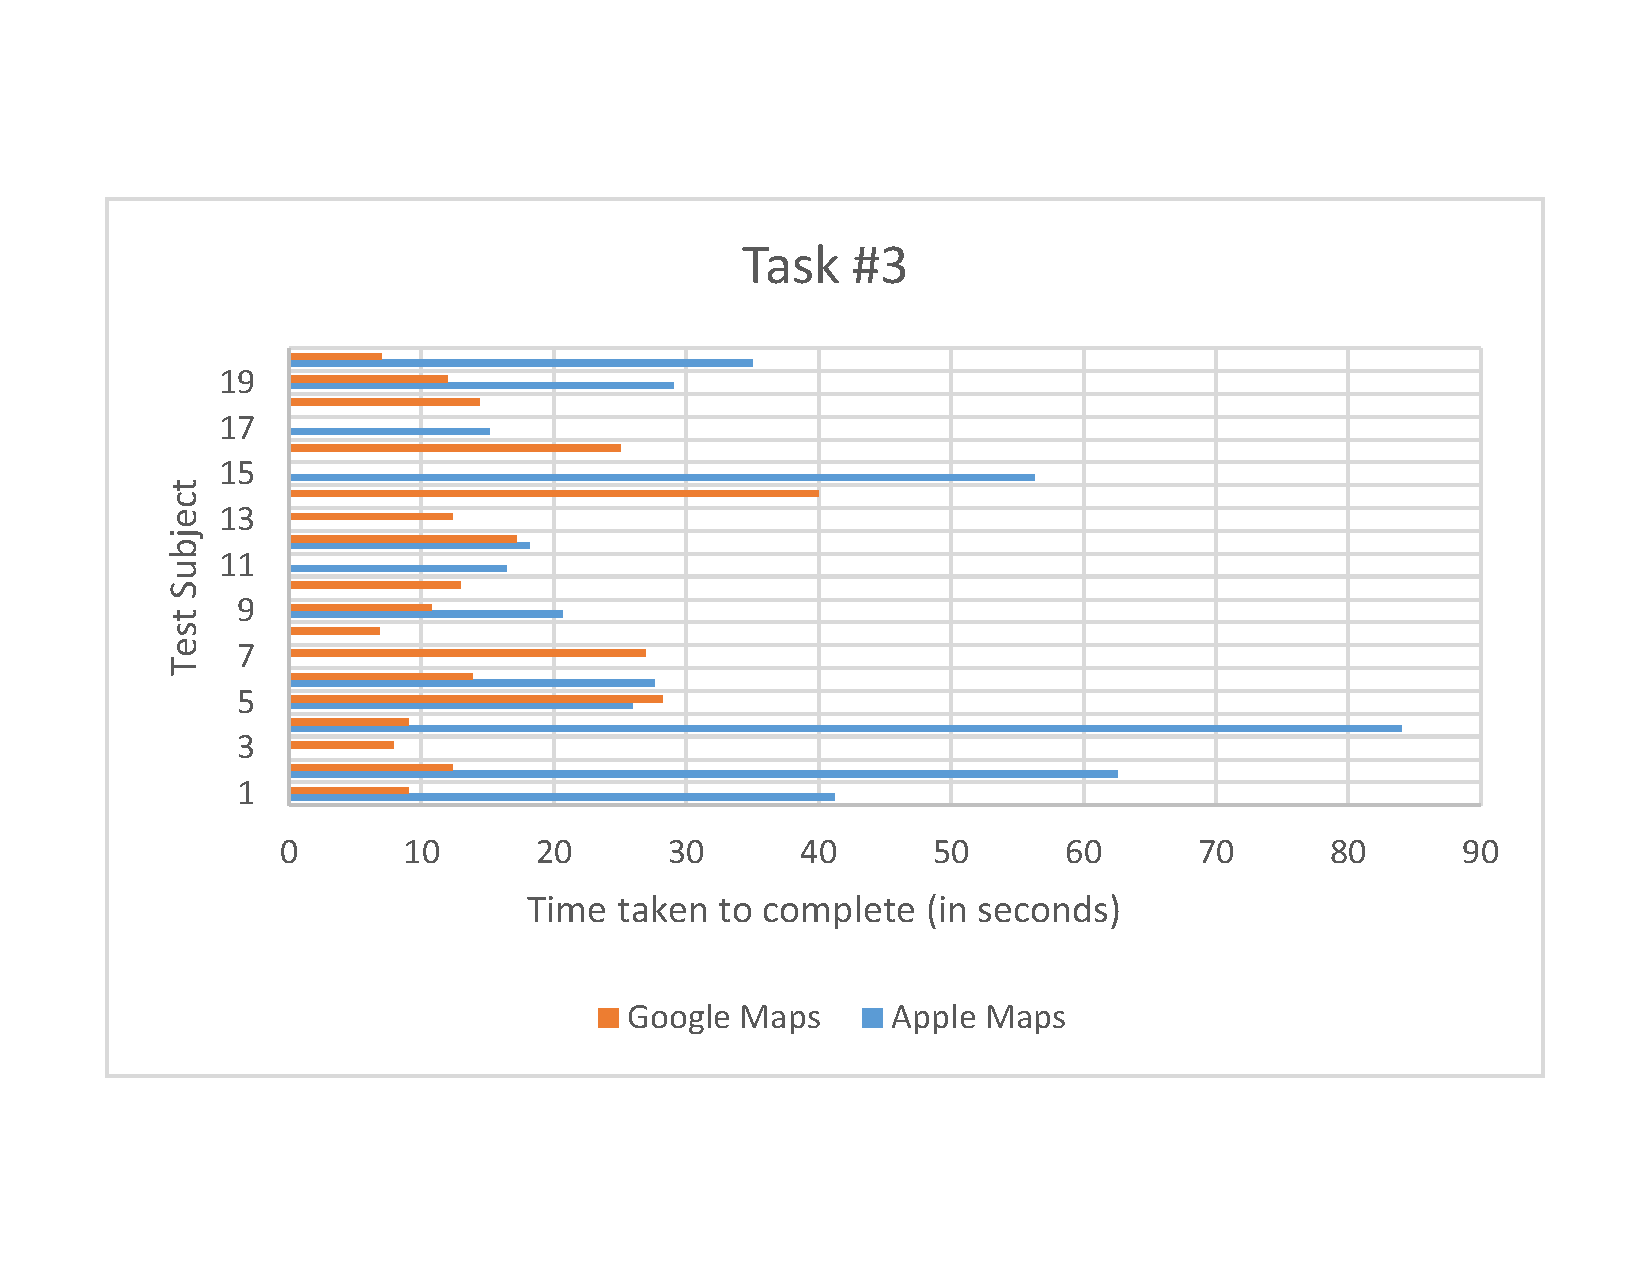
\includegraphics[keepaspectratio, width=1\textwidth ]{task3.pdf}
\end{figure}

\begin{table}[ht]
\centering 
\begin{tabular}{l c c c c c c c} % The final bracket specifies the number of columns in the table along with left and right borders which are specified using vertical bars (|); each column can be left, right or center-justified using l, r or c. To specify a precise width, use p{width}, e.g. p{8cm}
& \multicolumn{5}{c}{Map Application Tasks} \\ % Amalgamating several columns into one cell is done using the \multicolumn command as seen on this line
& Task1 & Error1 & Task2 & Error2 & Task3 & Error3 \\
User1 & 0.962 & 0.821 & 0.356 & 0.682 & 0.801\\ % Content row 1
NWN652 & 0.981 & 0.891 & 0.527 & 0.574 & 0.984\\ % Content row 2
PPD234 & 0.915 & 0.936 & 0.491 & 0.276 & 0.965\\ % Content row 3
JSB126 & 0.828 & 0.827 & 0.528 & 0.518 & 0.926\\ % Content row 4
JSB724 & 0.916 & 0.933 & 0.482 & 0.644 & 0.937\\ % Content row 5


Average Rate & 0.920 & 0.882 & 0.477 & 0.539 & 0.923\\ % Summary/total row

\end{tabular}
\caption{Table caption text}
\end{table}

\begin{table}
\centering
\begin{tabular}{l|r}
Item & Quantity \\\hline
Widgets & 42 \\
Gadgets & 13
\end{tabular}
\caption{\label{tab:widgets}An example table.}
\end{table}


\begin{multicols}{2}
[
\section{First Section}
All human things are subject to decay. And when fate summons, Monarchs must obey.
]
Hello, here is some text without a meaning.  This text should show what 
a printed text will look like at this place.
If you read this text, you will get no information.  Really?  Is there 
no information?  Is there...
\end{multicols}
\clearpage
\begin{thebibliography}{100} % 100 is a random guess of the total number of 
%references
\bibitem{Nielsen} Nielsen, Jakob, \emph{Usability Engineering}, Boston: Academic, 1993.
\bibitem{Mossberg} Mossberg, Walt., ``The iPhone Takes to the Big Screen," \emph{The Wall Street Journal}, September 2012.
\bibitem{ComScore}``Analytics for a Digital World - ComScore, Inc." \emph{ComScore,Inc}, 2012.
\bibitem{HK} Kopka, H., Daly P.W., \emph{A Guide to LaTeX},
Addison-Wesley, Reading, MA, 1999.
\bibitem{Pan} Pan, D., ``A Tutorial on MPEG/Audio Compression," \emph{IEEE 
Multimedia}, Vol.2, pp.60-74, Summer 1998.
\end{thebibliography}
%%%%%%%%%%%%% end %%%%%%%%%%%%%%%%%%%%%%%%%%%%%%%



\end{document}